\documentclass[tikz,border=4pt]{standalone}
\usepackage[T1]{fontenc}
\usepackage{mathptmx}
\usetikzlibrary{arrows.meta,calc}
\begin{document}
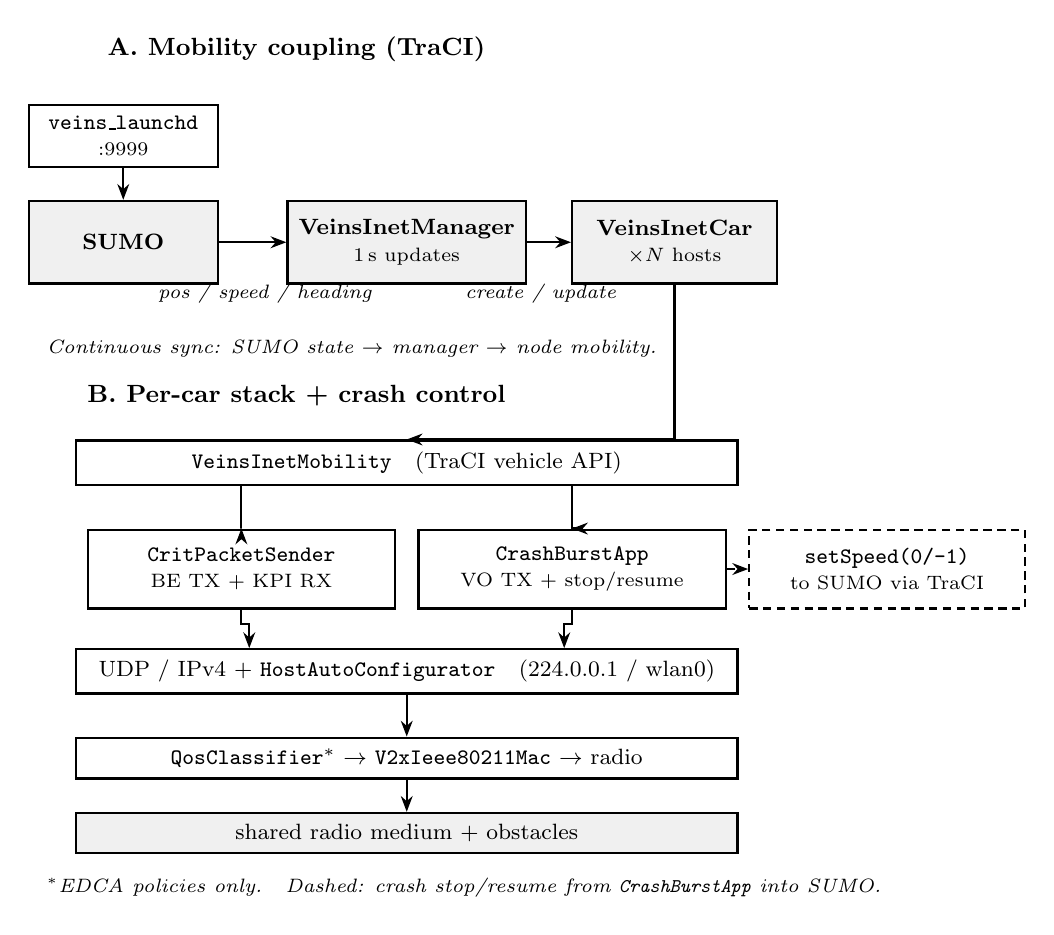
\begin{tikzpicture}[
  font=\footnotesize,
  >=Stealth,
  thick,
  box/.style={draw, thick, align=center, inner sep=4pt},
  panel/.style={box, fill=black!6},
  stack/.style={box, fill=white},
  title/.style={font=\small\bfseries},
  note/.style={font=\scriptsize\itshape, align=center},
  arr/.style={-{Stealth[length=2.0mm]}, thick},
]
  % ===== A. Mobility coupling =====
  \node[title] at (2.2,4.55) {A.\ Mobility coupling (TraCI)};

  \node[stack, minimum width=2.4cm] (launchd) at (0.0,3.45)
    {\texttt{veins\_launchd}\\{\scriptsize :9999}};
  \node[panel, minimum width=2.4cm, minimum height=1.05cm] (sumo) at (0.0,2.1)
    {\textbf{SUMO}};
  \node[panel, minimum width=2.8cm, minimum height=1.05cm] (mgr) at (3.6,2.1)
    {\textbf{VeinsInetManager}\\{\scriptsize 1\,s updates}};
  \node[panel, minimum width=2.6cm, minimum height=1.05cm] (carN) at (7.0,2.1)
    {\textbf{VeinsInetCar}\\{\scriptsize $\times N$ hosts}};

  \draw[arr] (launchd) -- (sumo);
  \draw[arr] (sumo) -- (mgr);
  \draw[arr] (mgr) -- (carN);
  \node[note] at (1.8,1.45) {pos / speed / heading};
  \node[note] at (5.3,1.45) {create / update};
  \node[note, anchor=west] at (-1.1,0.75)
    {Continuous sync: SUMO state $\rightarrow$ manager $\rightarrow$ node mobility.};

  % ===== B. Per-car stack =====
  \node[title] at (2.2,0.15) {B.\ Per-car stack + crash control};

  \node[stack, minimum width=8.4cm] (mob) at (3.6,-0.7)
    {\texttt{VeinsInetMobility}\quad (TraCI vehicle API)};

  \node[stack, minimum width=3.9cm, minimum height=1.0cm] (app0) at (1.5,-2.05)
    {\texttt{CritPacketSender}\\{\scriptsize BE TX + KPI RX}};
  \node[stack, minimum width=3.9cm, minimum height=1.0cm] (app1) at (5.7,-2.05)
    {\texttt{CrashBurstApp}\\{\scriptsize VO TX + stop/resume}};
  \node[stack, minimum width=3.5cm, densely dashed, minimum height=1.0cm] (crash) at (9.7,-2.05)
    {\texttt{setSpeed(0/-1)}\\{\scriptsize to SUMO via TraCI}};

  \node[stack, minimum width=8.4cm] (ip) at (3.6,-3.35)
    {UDP / IPv4 + \texttt{HostAutoConfigurator}\quad (224.0.0.1 / wlan0)};
  \node[stack, minimum width=8.4cm] (mac) at (3.6,-4.45)
    {\texttt{QosClassifier}$^\ast$ $\rightarrow$ \texttt{V2xIeee80211Mac} $\rightarrow$ radio};
  \node[panel, minimum width=8.4cm] (med) at (3.6,-5.4)
    {shared radio medium + obstacles};

  \draw[arr] (carN.south) -- ++(0,-0.45) |- (mob.north);
  \draw[arr] (mob.south) ++(-2.1,0) |- (app0.north);
  \draw[arr] (mob.south) ++(2.1,0) |- (app1.north);
  \draw[arr, densely dashed] (app1) -- (crash);
  \draw[arr] (app0.south) -- ++(0,-0.18) -| ($(ip.north)+(-2.0,0)$);
  \draw[arr] (app1.south) -- ++(0,-0.18) -| ($(ip.north)+(2.0,0)$);
  \draw[arr] (ip) -- (mac);
  \draw[arr] (mac) -- (med);

  \node[note, anchor=west, align=left] at (-1.1,-6.1) {%
    $^\ast$EDCA policies only.\quad
    Dashed: crash stop/resume from \texttt{CrashBurstApp} into SUMO.};
\end{tikzpicture}
\end{document}
